\documentclass[journal]{IEEEtran}
%
% If IEEEtran.cls has not been installed into the LaTeX system files, manually specify the path to it like:
% \documentclass[journal]{../sty/IEEEtran}

\usepackage{balance} % for balancing columns on the final page
% \usepackage{booktabs} % For formal tables
\usepackage{graphics} % for pdf, bit-mapped graphics files
\usepackage{epsfig} % for postscript graphics files
\usepackage{mathptmx} % assumes new font selection scheme installed
\usepackage{times} % assumes new font selection scheme installed
\usepackage{amsmath} % assumes amsmath package installed
\usepackage{amssymb}  % assumes amsmath package installed
% \usepackage{booktabs} % For formal tables
\usepackage{graphicx}
\usepackage{subcaption}
\usepackage{hyperref}

% mark the beginning of document
\begin{document}

% paper title
\title{This is a Sample LaTeX Document}

%author
\author{Judhi Prasetyo, M00609881, j.prasetyo@mdx.ac.ae}


% make the title area
\maketitle

% As a general rule, do not put math, special symbols or citations
% in the abstract or keywords.
\begin{abstract}
Collective decision-making is a process where individuals in a swarm have to reach consensus on a decision using only local interactions without any centralized or external control. In the context of the best-of-$n$ problem - whereby the consensus on the best option among a set of $n$ alternative is sought - it has been shown that consensus to one option (e.g. the best one) can be reached if individuals disseminate that option more than the others.
Besides being used as a mechanism to modulate positive feedback to achieve good collective decision, long dissemination times could potentially also been used in an adversarial way, whereby adversarial swarms could infiltrate the system and propagate bad decisions using aggressive dissemination strategies. Motivated by the above scenario, in this paper we propose a bio-inspired defence strategy that allows the swarm to be resilient against options that can be disseminated for longer times. This strategy mainly consists in reducing the mobility of the agents that are associated to options that can be disseminated for a shorter amount of time, allowing the swarm to converge to this option. 
We study the effectiveness of this strategy using two classical decision mechanisms, the voter model and the majority rule, showing that the majority rule is, at least in the current setting, necessary for this strategy to work. The strategy has also been validated on a real Kilobots proof of concept experiment. 
\end{abstract}

\begin{IEEEkeywords}
Collective decision-making, Best-of-n problem, spatial defence
\end{IEEEkeywords}


\section{Introduction}
% The very first letter is a 2 line initial drop letter followed
% by the rest of the first word in caps.
\IEEEPARstart{F}{or} the past few years, swarm robotics is getting momentum, thanks to the availability of cheaper and smaller agents, with available integrated sensors and communication devices~\cite{book:Hamann:2018}.  While  swarms of robots that are either manually controlled or operated semi-autonomously using external sensing and/or computation are nowadays well established, the realization of fully autonomous swarms of robots, with sensing and computation realized fully on-board, is still under investigation. The field of swarm robotics defines a swarm as a potentially large group of robots that operate without any centralized or external control, but by only relying on local interaction and communication~\cite{brambilla|ferrante|birattari|dorigo:2013}. Swarms of robots are potentially very beneficial mostly  in GPS denied environment, where the external control is prevented by the unavailability of communications or GPS. 


\begin{figure*}[t]
  \centering
  \subfloat[]{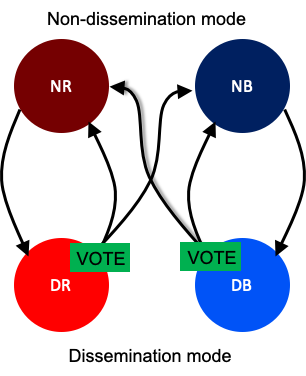
\includegraphics[width=0.3\textwidth]{images/StateMachine.png}
  \label{fig:statemachine}}
  \hfill
  \subfloat[]{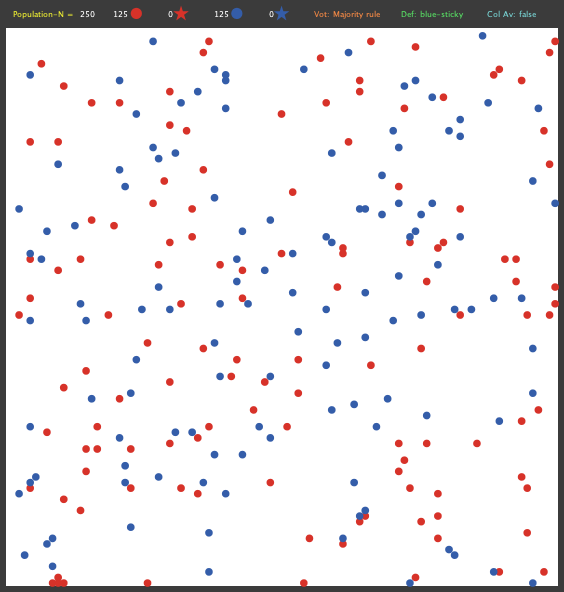
\includegraphics[width=0.4\textwidth]{images/arena.png}
  \label{fig:arena}}
  \hfill
  \caption{Panel $a$: Probabilistic finite state machine. $NR$, $NB$ , $DR$  and $DB$ represent the non-dissemination and dissemination states, for RED and BLUE agents respectively.  Panel $b$: Screenshot of the simulation arena. %This image is taken from NetLogo software
  }
  \label{fig:arena_and_method}
\end{figure*}

\subsection{Collective Decision Making}
One of the basic capability sought in a robot swarm is attainment of collective decisions~\cite{book:Bonabeau1999SwarmI,Valentini2017Review}. Many other collective behaviours can be seen as an instance of collective decision making, such as deciding a common direction of motion~\cite{FerranteNOALIGN}, or a common location in the environment to explore at~\cite{correll|martinoli:2011}. A special case of collective decision making is represented by the best-of-$n$ problem, whereby there is a discrete number $n$ of options and the swarm has to achieve consensus on the best of them. A  perspective on the best-of-$n$ problem can be found in~\cite{Valentini2017Review}, whereby it is argued that two factors are key in collective decision-making: the intrinsic qualities associated to the different options~\cite{FontLlenas:ANTS:2018,valentini|hamann|dorigo:2014,valentini|ferrante|hamann|dorigo:2015}, or the cost associated to each option in case of asymmetrical environments~\cite{montesdeoca|ferrante|scheidler|pinciroli|birattari|dorigo:2011,scheidler|brutschy|ferrante|dorigo:2015,BruSchFer-etal2012:iros}. In this view, the \emph{best} option the swarm has to choose can be the one associated to the highest quality, to the lowest cost, or a compromise between these two.

\subsection{Positive Feedback Modulation}
In general, across all those cases, the key factor determining to what option the swarm will converge is positive feedback: if robots observe, on average, more frequently one option, the swarm will more likely converge to this option. This happens because the initial symmetry (equal distribution of options) will more likely break in favour of the most frequently observed option, and subsequently this option will be even more abundant (positive feedback), thus biasing even further the consensus, and so on. This "frequency of exposure", or modulation of positive feedback, for one option can be environment-dependent and uncontrolled (passive modulation of positive feedback) in case of asymmetric environmental cost (e.g. in tasks in which the physical path to each option differs~\cite{montesdeoca|ferrante|scheidler|pinciroli|birattari|dorigo:2011}), or can be instead controlled by modulating the frequency of dissemination (active modulation of positive feedback, e.g. via communication) as a control parameter, for example by having it proportional to the quality of the option assuming it can be measured~\cite{valentini|ferrante|hamann|dorigo:2015}. While in general the best-of-$n$ collective decision making is not adapting to sudden changes of the environments, it has been demonstrated that such adaptability can be achieved by introducing a  limited number of stubborn individuals~\cite{prasetyo2018, DeMasiHTC2020}. 

\section{PROBLEM DEFINITION AND METHOD}
\label{sec:method}


\begin{table*}[t]
\caption{Experiment Parameters}
\label{params-table}
\centering
\begin{tabular}{|c|c|c|}
\hline
Notation & Values &
Description
\\
\hline
$N$
&
$[100, 250, 500, 750, 1000]$.
&
Swarm Population, total number of robots.\\
\hline
$\rho_{RED}$
&
$[1.0, 1.25, 2.5, 3.75, 5.0, 6.25, 7.5, 8.75, 10]$
&
RED Dissemination Factor.\\
\hline
$\rho_{BLUE}$
&
$[1.0]$
&
BLUE Dissemination Factor.\\

\hline
-
&
["Voter Model","Majority Rule"]
&
Voting methods.
\\
\hline
$k$
&
$[3,5,7]$
&
Minimum number of agents that participate in the voting when using Majority Rule.
\\
\hline
\end{tabular}
\end{table*}


We consider a collective decision making-process in a swarm of $N$ agents modeled as the discrete best-of-$n$~\cite{Valentini2017Review}. We consider the case $n=2$, and we label the two options as RED and BLUE. The two options are associated to different dissemination times: the RED option is the \emph{attacker} option and has a longer dissemination time than the BLUE option, the \emph{defender} option.

The dissemination times above are exponentially distributed and each (BLUE or RED) proportional to a parameter that we call \emph{dissemination factor}.  Only the ratio between the two dissemination factors play a role. %, rather then their absolute values [CITARE]. 
To keep the observation simple, the dissemination factor of BLUE has been fixed to the value $1$. Only the RED dissemination factor $\rho_{RED}$ is varied, using values greater or equal to $1$. 
Half of the population is initialized with RED opinion and the other half with BLUE opinion. 
% answer to Review  1-2 below
Agents with RED opinion have dissemination time  proportional to RED option value, and those with BLUE opinion will disseminate proportional to BLUE option value.  
The agents' location are initially randomly distributed.

The agents with the RED opinion implement a random walk and always move freely in an arena with closed bounds and no periodic boundaries. When they do not implement any strategy (here referred to as \emph{No Strategy}), the BLUE agents perform random walk exactly like the agents with the RED option. But, when they implement our novel defence strategy (referred to as \emph{Blue-sticky}), they remain in their initial position. If a RED robot changes opinion after the decision making mechanism, it becomes BLUE  and stops in its last position.  Within the simulations, collision checks are not implemented and individuals may freely collide or overlap with each other, an assumption that does not hold in the real robot experiments.

\section{Experiment}
The robot behavior can be modeled as a Finite State Machine in Fig. \ref{fig:statemachine}. All agents start in a non-dissemination state (NR or NB, for RED and BLUE respectively) and they remain in this state for an  amount of time that is randomly sampled from an exponential distribution with parameter $\tau_{ND} = q = 10$, common to RED and BLUE agents.
Then they transition to a dissemination state (DR or DB), in which they promote their opinion for an amount of time sampled from an exponential distribution with parameter proportional to the dissemination factor $\tau_D= q \cdot \rho_i$, where $q=10$  and  $i \in \{ RED, BLUE \}$, after which they perform \emph{voting} before transitioning again to non-dissemination mode and the cycle repeats. %The rate of the dissemination time for the RED (resp. BLUE) option is equal to \textbf{write}. 
Since, as explained above, we only consider $\rho_{RED} > \rho_{BLUE} = 1$, the dissemination time for the RED option is on average larger than the dissemination time of the BLUE option. In absence of defence mechanisms, this is shown to lead to a positive feedback modulation mechanism that makes the system converge to the RED option with higher probability compared to the BLUE option~\cite{valentini|ferrante|hamann|dorigo:2015}. 

Lorem ipsum dolor sit amet, consectetur adipiscing elit, sed do eiusmod tempor incididunt ut labore et dolore magna aliqua. Lectus quam id leo in vitae turpis. In est ante in nibh. Enim ut sem viverra aliquet eget sit amet tellus cras. Aliquam etiam erat velit scelerisque in dictum non. Dictum sit amet justo donec enim diam. Tristique sollicitudin nibh sit amet commodo nulla facilisi nullam. A arcu cursus vitae congue mauris. Fermentum leo vel orci porta non pulvinar neque. Eu scelerisque felis imperdiet proin fermentum leo vel orci porta. Senectus et netus et malesuada fames ac turpis egestas integer. Facilisis mauris sit amet massa vitae tortor condimentum lacinia quis. Eget nulla facilisi etiam dignissim diam quis.

Tincidunt id aliquet risus feugiat in. Varius morbi enim nunc faucibus a pellentesque sit amet porttitor. In aliquam sem fringilla ut morbi tincidunt augue. Dui vivamus arcu felis bibendum ut tristique et egestas. Duis ultricies lacus sed turpis. Sed sed risus pretium quam vulputate dignissim. Consectetur adipiscing elit pellentesque habitant. Arcu odio ut sem nulla pharetra diam sit. Eu consequat ac felis donec. Arcu bibendum at varius vel pharetra. Vulputate odio ut enim blandit volutpat maecenas volutpat blandit aliquam. Augue lacus viverra vitae congue eu consequat ac felis donec. 

This is an example sentence that refer to a figure~\ref{fig:chart} that should be automatically shown before this paragraph, although it is defined after.

\begin{figure}
  \centering
  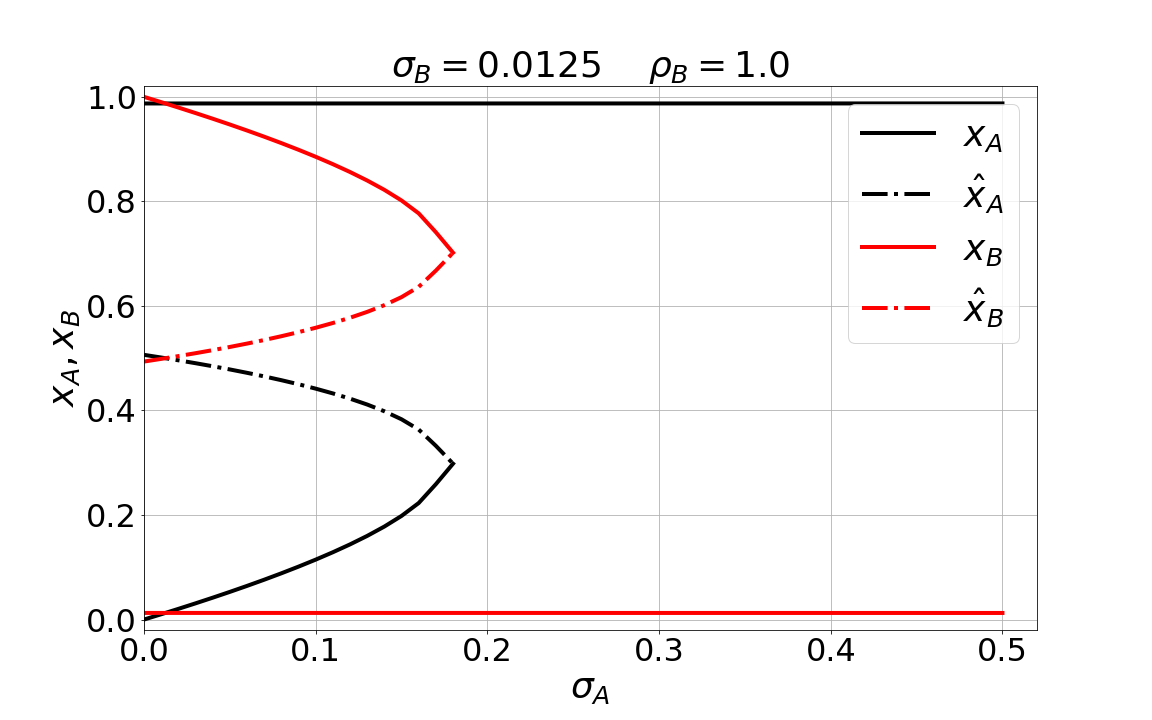
\includegraphics[width=0.3\textwidth]{images/chart.png}
  \hfill
\caption{Only one figure in a single column}
  \label{fig:chart}
\end{figure}


\section{Conclusion}
In this paper, we study a mechanism to increase the resiliency of a swarm of agents performing collective decision making, subject to attacks represented by the malicious exploitation of the positive feedback modulation. Two options, BLUE and RED, are assumed to have two different dissemination factors, that is two different times of dissemination of their opinions. The BLUE option is characterized by a dissemination factor that is lower than the RED option. Nevertheless, the BLUE option wants to defend its opinion, against the attacks of the RED option. The BLUE option can still win the consensus, when the agents with such opinion use a  spatial strategy through which they stay in place and stick the attacker, once it is converted from RED to BLUE. 
This mechanism is  inspired by the defence strategy used by stingless bees, that use some special resin to stick attackers in order to defend themselves. 

We can conclude that, if agents are attacked by more aggressive agents (with higher dissemination factor), a good strategy for them to win is to stop where they are and progressively form clusters. This study can be particularly relevant for patrolling and surveillance applications. The fact that small systems are more resilient to external attacks, compared with larger systems make this strategy suitable to be applied in real surveillance swarms of agents. 

In the next studies, we will investigate the spatial distribution of agents, where agglomeration of blue agents is expected.  Finally, we note that the Blue-sticky can be considered a rudimentary aggregation behaviour, as it produces clusters, thus it is in our agenda to study the coupling of collective decision making with other collective behaviours that prouce different spatial correlations, such as collective motion or pattern formation. 

\begin{table}
\centering
\begin{tabular}{|p{0.1\textwidth}|p{0.3\textwidth}|}
\hline
No & Description \\
\hline
$1$ & One \\
$2$ & Two \\
$3$ & Three \\
\hline
\end{tabular}
\caption{Single column width table}
\end{table}


% use section* for acknowledgment
\section*{Acknowledgment}
We acknowledge Middlesex University Dubai for the lab facilities provided for Kilobots experiments.

% bibliography 
\bibliographystyle{plain}
\bibliography{biblio}

\end{document}

